
\documentclass{article}
\usepackage[margin=1.4in]{geometry}
\usepackage{color}
\usepackage{caption}
\usepackage{hyperref}
\usepackage{csquotes}
\usepackage{amsmath}
\usepackage{amssymb}
\usepackage{soul}
\usepackage{changepage}
\usepackage{alg}
\usepackage{graphicx}
\graphicspath{ {./} }
\usepackage{listings}
\lstset{aboveskip=3mm, belowskip=3mm, showstringspaces=false, columns=flexible, basicstyle={\small\ttfamily}, numbers=none, breaklines=true, breakatwhitespace=true, tabsize=3}

\usepackage{newlfont}
\usepackage{program}
\catcode`\_\active

\newtheorem{randlang}{RandLang}[section]

\begin{document}
\begin{center}{\huge   Lab 2: Random Walks with Chemotaxis }\\[0.4cm]{\large  Philosophy of Computation }\\[0.75cm]{\large  Henry Blanchette }\\[0.5cm]{\large  February 22st, 2019 }\\[1.0cm]\end{center}\section{Introduction}


  A \textit{random walk} is a random path through some mathematical space $  X  $. A walk is generated by an implementation of the following generic algorithm:



  \vspace{0.4cm}
  \subsubsection*{The Random Walk Specification}

\begin{adjustwidth}{1cm}{}\begin{programbox}
steps \in \mathbb{N} := \mbox{the number of steps to take}
x \in X := \mbox{the start point}
\FOR 1 \TO steps \DO
  \vec{\theta} := \mbox{a randomly chosen unit vector}
  l := \mbox{a randomly chosen length}
  x := x + l \vec{\theta}
\OD
\end{programbox}\end{adjustwidth}
 \vspace{0.6cm}


  The idea is that an ``agent'' begins their journey at $  x  $, and then for each of $  steps  $ times the agent takes a random step from $  x  $ to a new position. A specific implementation describes the choosing of $  l, \vec{\theta}  $, and the space in which the walk occurs.


\subsection{Random Walks in One Dimension}


  In one dimension, random walks are very simple. The following algorithm describes a random walk $  \mathbb{R}  $ in terms of some configurable parameters:



  \vspace{0.4cm}
  \subsubsection*{Random Walk in $\mathbb{R}$}

\begin{adjustwidth}{1cm}{}\begin{programbox}
steps := \mbox{the number of steps to take}
\textit{step-maximum} := \mbox{the maximum step size}
x \in \R := \mbox{the start point}
\FOR 1 \TO steps \DO
  \vec{\theta} := \mbox{chosen uniformly from } \{-1,1\}
  l := \mbox{chosen uniformly in } [0, \textit{step-maximum}]
  x := x + l \vec{\theta}
\OD
\end{programbox}\end{adjustwidth}
 \vspace{0.6cm}


  But what does this kind of walk look like? A useful metric with which to analyze random walks is the distribution of their endpoints after some number of steps. Figure 1 is a histogram of the endpoints of 10,000 random walks on $  \mathbb{R}  $ after 1,000 steps each, with a \textit{step_maximum} of 1.



\begin{figure}[h]
\centering
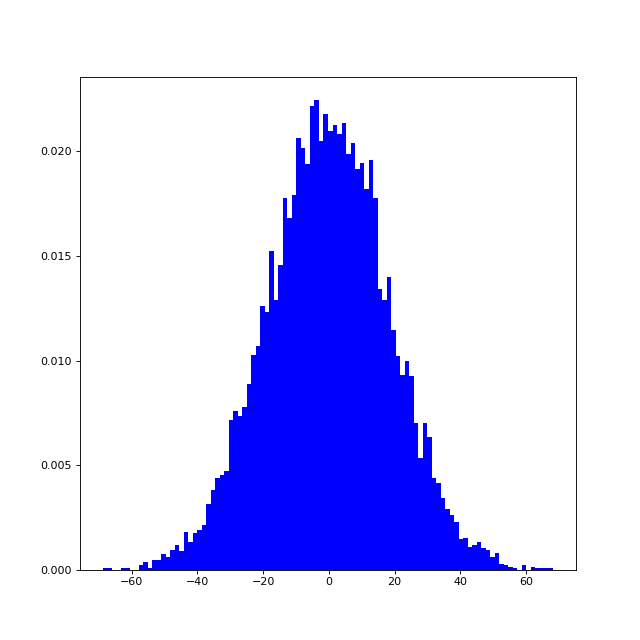
\includegraphics[width=10cm,keepaspectratio]{images/walk1d-hist.png}
\captionsetup{labelformat=empty} \caption{Figure 1. Distribution of endpoints for 10,000 random walks in $\mathbb{R}$ after 1,000 steps each.}
\end{figure}



  This familiar shape is, in fact, a Gaussian distribution. The variance of \textit{steps} and \textit{step_maximum} will correspond to a change in the distributions generating $  \sigma  $, and the \textit{start-point} corresponds to the distribution's mean.


\subsection{Random Walks in Two Dimensions}


  Are random walks in $  \mathbb{R}^2  $ any different from those in $  \mathbb{R}  $? First of all, the generating algorithm is as follows:



  \vspace{0.4cm}
  \subsubsection*{Random Walk in $\mathbb{R}^2$}

\begin{adjustwidth}{1cm}{}\begin{programbox}
steps := \mbox{the number of steps to take}
\textit{step-maximum} := \mbox{the maximum step size}
x \in \mathbb{R}^2 := \mbox{the start point}
\FOR 1 \TO steps \DO
  \vec{\theta} := (\cos \theta, \sin \theta) \mbox{ where $\theta$ is chosen uniformly from } [0, 2\pi)
  l := \mbox{chosen uniformly in } [0, \textit{step-maximum}]
  x := x + l \vec{\theta}
\OD
\end{programbox}\end{adjustwidth}
 \vspace{0.6cm}


  Again, we can look at the distribution of the endpoints of such walks after some number of steps. Figure 2 depicts the distribution of endpoints for 10,000 walks each after 1,000 steps.



\begin{figure}[h]
\centering
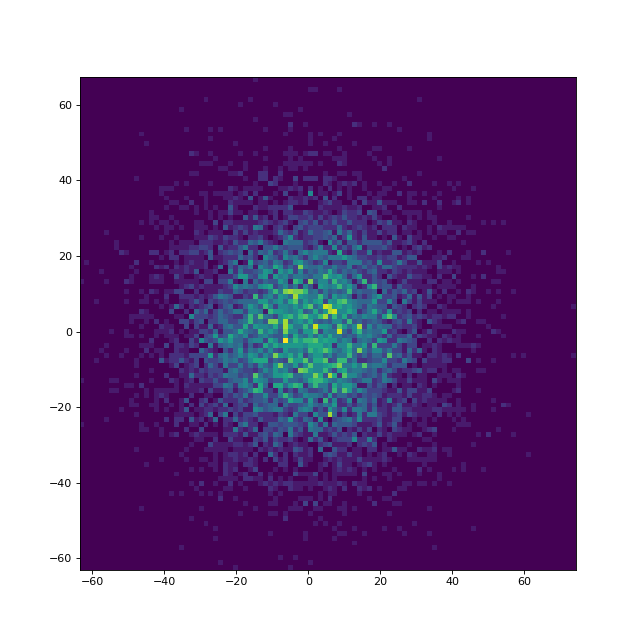
\includegraphics[width=10cm,keepaspectratio]{images/walk2d-hist.png}
\captionsetup{labelformat=empty} \caption{Figure 2. Distribution of endpoints for 10,000 random walks in $\mathbb{R}^2$ after 1,000 steps each.}
\end{figure}



  The result is analogous to the 1-dimensional walk: the distribution is Gaussian again.


\section{Chemotaxis}


  Chemotaxis are the mechanisms that some bacteria use to move around in a medium. Chemotaxis allow a bacterium to explore an environment in a pseudo-random manner, biased by some sensor the bacteria uses to locate a sought resource such as sugar.


\subsection{Chemotaxi Mechanisms}


  Bacteria using chemotaxis have several components that work together to allow non-uniformly-random movement. The bacteria have flagella can be swung at an angle, making the bacteria either move forward streamlined through the medium or rotating in place. Moving forward is termed \textit{running} and rotating in place is termed \textit{tumbling}. The chemotaxi strategy is a mixture of running and tumbling.



\begin{figure}[h]
\centering
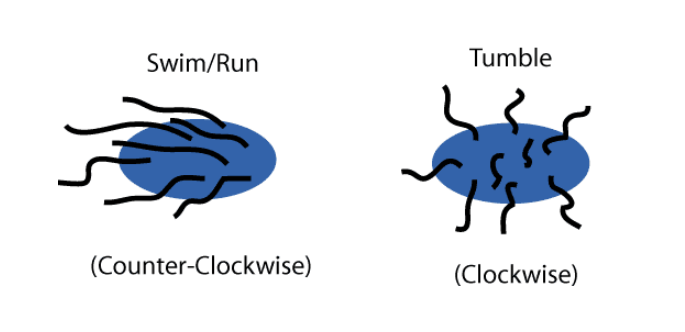
\includegraphics[width=10cm,keepaspectratio]{images/chemotaxi-mechanisms.png}
\captionsetup{labelformat=empty} \caption{Figure 3. A visual depiction of chemotaxis in action. Flagella pivot relative to their roots on a bacterium to interact with the medium and either run or tumble.}
\end{figure}



  Note that running and tumbling combine together to give an implementation of the general random walk algorithm: A tumble chooses a new orientation ($  \vec{\theta}  $) for the bacterium, and a run will propel it forward some distance ($  l  $) in that direction.


\subsection{Biased Random Walks}


  So far, our random walks have made use of uniform randomness when choosing $  \vec{\theta}, l  $. A biased random walk is one where these choices are made using some non-uniform weighting over their respective domains. In the bacteria world, a variant of randomly walking becomes very useful. The capabilities of bacterial movement are, clearly, very crude and so a biased random walk turns out to well simulate the process that chemotaxis implement in reality.


\section{Simulation}


  The common situation we will simulate is where the bacteria is positioned in $  \mathbb{R}^2  $ (for simplicity) and the space comes with a function $  food: \mathbb{R}^2 \rightarrow \mathbb{R}  $. $  food  $ maps each position in the space to the inverse of the concentration of food it contains. Bacteria's goal in this environment is to move, via chemotaxis, to the highest concentrations of food (where $  food  $ reaches a local minimum). The only sensor the bacteria have access to is a chemical equivalent of measuring the gradient of $  food  $ at their current location. In nature, the distribution of food is relatively smooth, and especially so in this simulation. Defined specifically, let's use


\begin{align*} 
  food:
  \mathbb{R}^2 &\rightarrow \mathbb{R} \\
  (x,y) &\mapsto (\delta_x^2 + \delta_y^2)^{1/6}
 \end{align*} \vspace*{0.1cm}


  where $  (\delta_x, \delta_y) := (x - x_0, y - y_0)  $ and $  (x_0, y_0)  $ is the \textit{center} of the distribution (which is defined for convenience and will be configured later). This definition yields the following gradient


\begin{align*} 
  \Delta_{food}:
  \mathbb{R}^2 &\rightarrow \mathbb{R} \\
  (x,y) &\mapsto
    \left(
      \frac{1}{6} 2 \delta_x (\delta_x^2 + \delta_y^2)^{-1/6},
      \frac{1}{6} 2 \delta_y (\delta_x^2 + \delta_y^2)^{-1/6}
    \right)
 \end{align*} \vspace*{0.1cm}


  I chose this Laplacian distribution in order to make the center of the distribution fairly spikey, as to be different from just a distribution that is just derived from the distance to the center (a cone).





  So, with this setup, the bacteria want to (somehow) travel in the direction in which the food gradient is least, as to head towards the minimum which is the center of the distribution. This mimics actual bacteria's sensory determination of the gradient of food (sugar) distribution.





  To achieve this goal, the bacteria will bias their choice of run distance ($  l  $) in the following way, given that they are at position $  (x,y)  $ and have already chosen (tumbled to) orientation $  \vec{\theta}  $:


\begin{align*} 
  l := \textit{step-maximum } \cdot (-\Delta_{food}(x,y) \times \vec{\theta} + 1) / 2
 \end{align*} \vspace*{0.1cm}


  A brief explanation --- the $  -\Delta_{food}(x,y) \times \vec{\theta}  $ gives the cosine of the angle between the gradient and the orientation, which is in the range $  [-1,1]  $, and then adding one and dividing by two puts the value in the range $  [0,1]  $. By the definition of cosine this value will maximize at 1 when the orientation is exactly towards the negative gradient (towards the food distribution center) and minimize at 0 when the orientation is exactly opposite the negative gradient, and vary smoothly between these extremes for other orientations.





  The resulting bias in the bacteria's walks is that they will run further ``downhill'' towards higher concentrations of food and shorted ``uphill'' away from higher concentrations of food. An example of batch of such chemotaxi walks is depicted in Figures 4 and 5.



\begin{figure}[h]
\centering
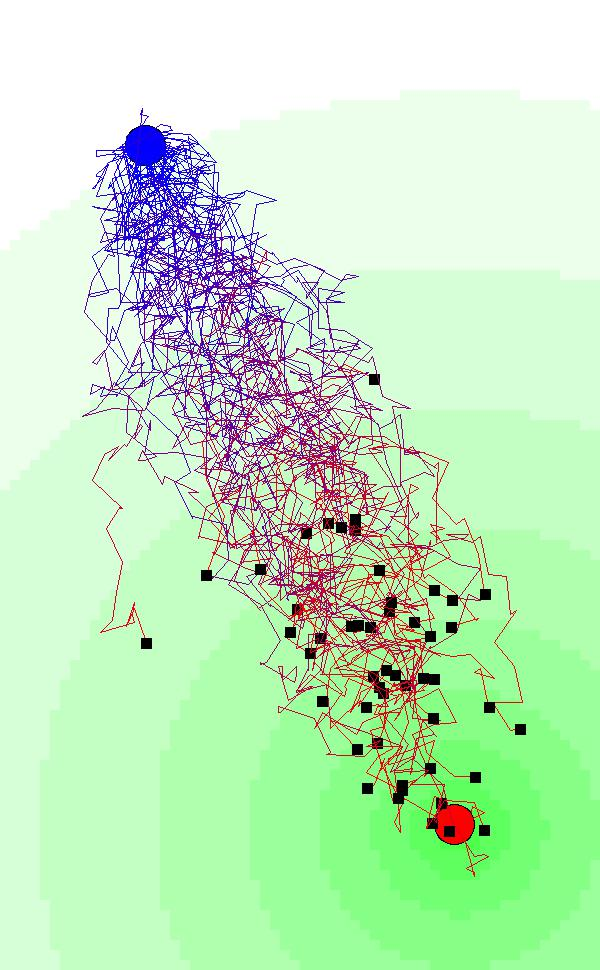
\includegraphics[width=10cm,keepaspectratio]{images/chemotaxi-paths-small.jpg}
\captionsetup{labelformat=empty} \caption{Figure 4. History of 50 chemotaxi walks each with 60 steps. The background green-scale shading indicates concentration of food. The large blue node marks the starting position for all the bacteria. The red node marks the center of the Laplacian distribution of food. For each walk, the steps are drawn in a shade that transitions from red to blue as the walk progresses. The black squares mark the endpoints for each of the walks.}
\end{figure}

\begin{figure}[h]
\centering
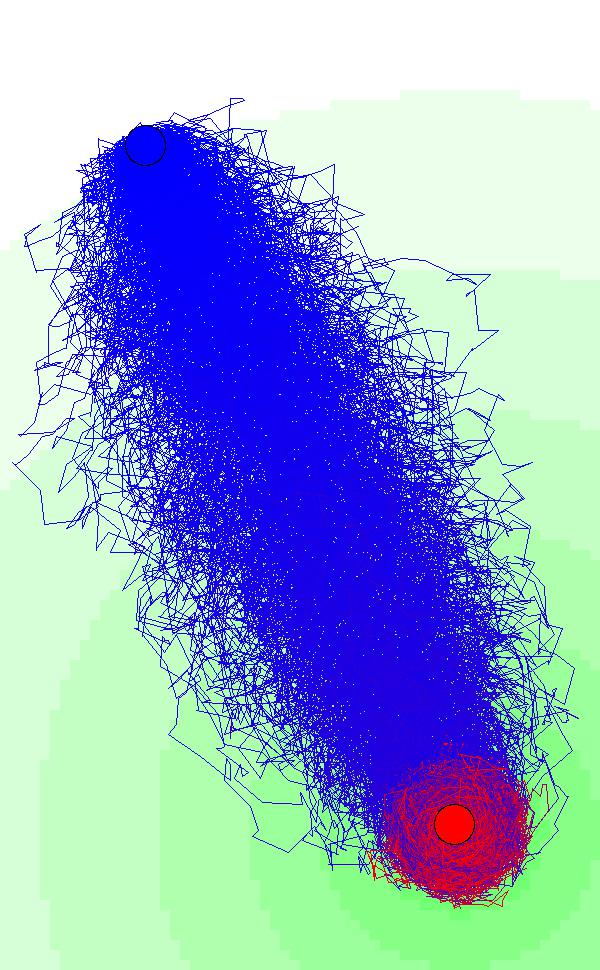
\includegraphics[width=10cm,keepaspectratio]{images/chemotaxi-paths-large.jpg}
\captionsetup{labelformat=empty} \caption{Figure 5. History of 500 chemotaxi walks each with 500 steps. The background green-scale shading indicates concentration of food. The large blue node marks the starting position for all the bacteria. The red node marks the center of the Laplacian distribution of food. For each walk, the steps are drawn in a shade that transitions from red to blue as the walk progresses. The black squares that would mark the endpoints for each of the walks have been omitted because they block visibility.}
\end{figure}



  As with the original random walks, it is also interesting to consider the distribution of endpoints after a given number of steps. Figures 6 and 7 show these histograms.



\begin{figure}[h]
\centering
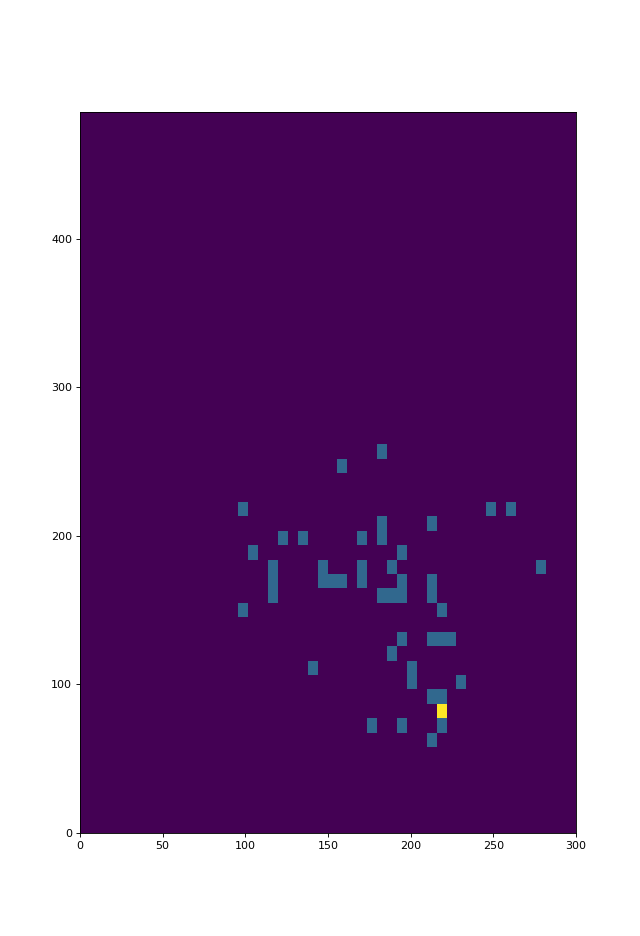
\includegraphics[width=10cm,keepaspectratio]{images/chemotaxi-histogram-small.png}
\captionsetup{labelformat=empty} \caption{Figure 5. Histogram of the endpoints of 50 chemotaxi walks each after 60 steps. The heat map is shaded by the concentration of endpoints in the corresponding bin.}
\end{figure}

\begin{figure}[h]
\centering
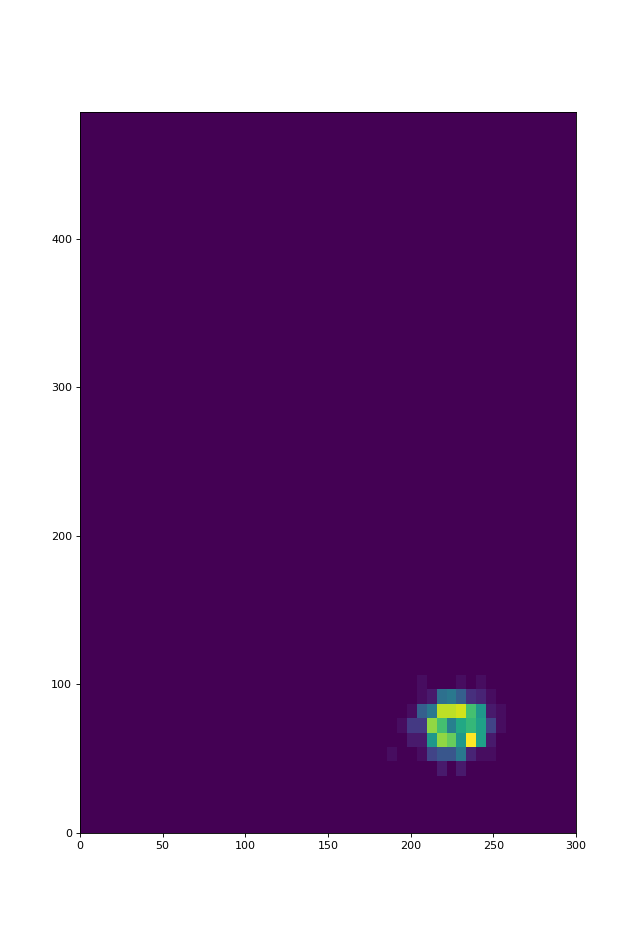
\includegraphics[width=10cm,keepaspectratio]{images/chemotaxi-histogram-large.png}
\captionsetup{labelformat=empty} \caption{Figure 6. Histogram of the endpoints of 500 chemotaxi walks each after 500 steps. The heat map is shaded by the concentration of endpoints in the corresponding bin.}
\end{figure}
\section{Conclusions}


  Random walks demonstrate a way for order to arise from chaos. The beginning of this report explored how mathematical random walks produce normal distributions in space over a variable radius from the walk origin, allowing for some locations in space (those closer to the walk origin) to be passed through more commonly than other locations (those further from the walk origin).





  The actions of chemotaxis, as a physical instantiation of a random walk, take advantage of this order-creating aspect of random walks to sustain bacteria through food-seeking. The bacteria themselves, of course, do not have an awareness or intent about the positioning of their flagella. The tumbling action models how the complexities of how bacteria randomly interact with the subtleties of their environment to, in effect, generate random orientations. As the chemotaxi strategy corresponds (roughly) to a random walk, chemotaxis combine this random interaction into the ordered emergent-behavior of moving through some positions in space more commonly than others. The sensor mechanism of chemotaxis, to measure the food concentration gradient at a bacterium's location, simply biases the already-ordered behavior of the random walk to ``center'' at the local minimum of food concentration.





  Bacteria are not the simplest examples of microscopic evolution in themselves; they employ versions of DNA that reflect an incorporation of a vast array of evolved complexities. But, at the level of treating each bacterium as atomic, the chemotaxi behavior seems to be a introductory level of higher-order evolution. Before having intent, bacteria have evolved chemotaxi mechanisms to dynamically sense, interact with, and respond to their environment. On the surface it is a process of input-output, but as a general phenomenon chemotaxi movement is clearly a larger-scale interaction between an agent and its environment that hints at the beginnings of an internal \textit{model} of the outer world that the bacteria's structure must encode.






\section*{Bibliography}


\noindent 
  Williams A. 2010. Chemotaxis on the move – active learning teaching tool. J. Microbiol. Biol. Educ. 11(2):177-178 doi:10.1128/jmbe.v11i2.216. 
\href{https://dx.doi.org/10.1128%2Fjmbe.v11i2.216}{[doi]}

\vspace*{0.2cm}


\noindent 
  Codling, Edward \& J Plank, Michael \& Benhamou, Simon. (2008). Random walks in biology. Journal of the Royal Society, Interface / the Royal Society. 5. 813-34. 10.1098/rsif.2008.0014. 
\href{https://doi.org/10.1098/rsif.2008.0014}{[dio]}

\vspace*{0.2cm}


\noindent 
  K.J. Duffy, P.T. Cummings, R.M. Ford, Random walk calculations for bacterial migration in porous media, Biophysical Journal, Volume 68, Issue 3, 1995, Pages 800-806, ISSN 0006-3495. 
\href{https://doi.org/10.1016/S0006-3495(95)80256-0}{[dio]}

\vspace*{0.2cm}
\end{document}